% Input common header
\documentclass[xcolor=dvipsnames]{beamer}

\usecolortheme[named=Blue]{structure}
\setbeamertemplate{itemize items}[circle]

\usepackage{smartdiagram}


\author{Dr. Paul Larsen}
\date{\today}

\usetikzlibrary{decorations}
\usetikzlibrary{snakes}

\title{Adversarial Regularization Regimes in Classification Tasks}
\begin{document}
\maketitle

\begin{frame}{Outline}
  \begin{itemize}
      \item What is adversarial machine learning?
      \item Classification algorithms with regularization
      \item Results for ridge regression and logistic regression
      \item Practical advice for data scientists
  \end{itemize}

  \vspace{2cm}
  Joint work with Maximilian Wiesmann, Max Planck Institute for Mathematics in the Sciences, Leipzig, Germany

\end{frame}

\begin{frame}{What is adversarial machine learning?}

  Ingredients of adversarial ML:

  \begin{itemize}
    \item an algorithm $f$ for prediction or classification
    \item a chosen or generated subset of input data $X \subset U$ such that $f(X)$ gives precisely the prediction or class
  \end{itemize}

\end{frame}


\begin{frame}{Adversarial ML example: fooling object classification algorithms}
  \begin{columns}[T] % align columns
    \begin{column}{.3\textwidth}

      \begin{center}
      \fbox{
        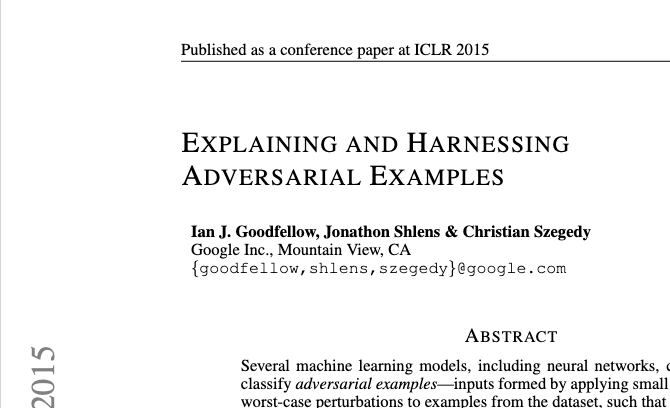
\includegraphics[width=1.\textwidth]{graphics/explaining-adversarial}
      }
      \end{center}
      \cite{goodfellow2014explaining}\newline

    \end{column}%
    \begin{column}{.7\textwidth}
      \begin{center}
        From pandas to gibbon ...
        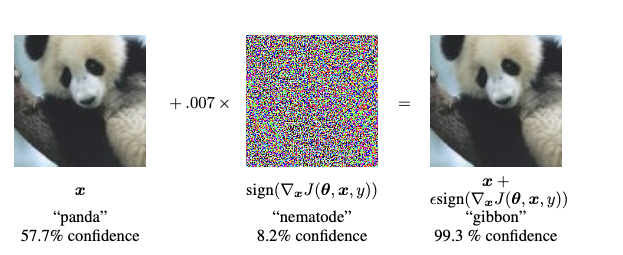
\includegraphics[width=0.7\textwidth]{graphics/gibbon-for-panda}
        \end{center}
    \end{column}%
\end{columns}
\end{frame}

\begin{frame}{Adversarial ML example: becoming invisible to object detection algorithms}
  \begin{columns}[T] % align columns
    \begin{column}{.3\textwidth}

      \begin{center}
      \fbox{
        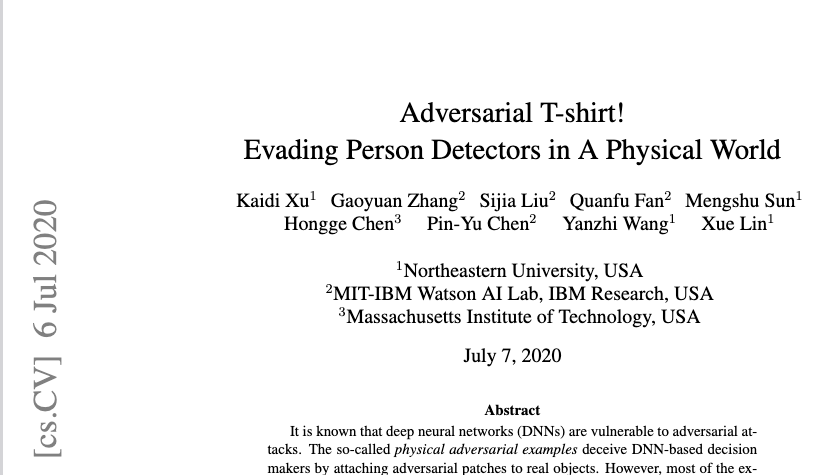
\includegraphics[width=1.\textwidth]{graphics/adversarial-tshirt}
      }
      \end{center}
      \cite{xu2020adversarial}\newline

    \end{column}%
    \begin{column}{.7\textwidth}
      \hspace{0.2\textwidth}It's like having your own cloaking device ...
      \begin{center}

        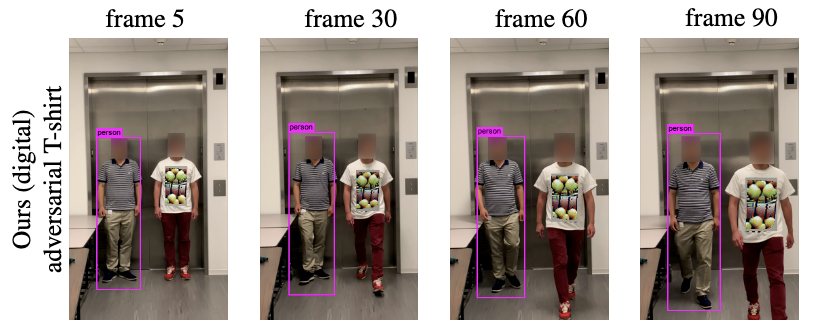
\includegraphics[width=0.7\textwidth]{graphics/cloaking-device}

        \end{center}
        \hspace{0.2\textwidth}You can \href{https://adversarial-designs.shop/collections/t-shirts-and-apparel}{buy your own}

        \hspace{0.2\textwidth}(No product endorsement implied)
    \end{column}%
\end{columns}
\end{frame}

\begin{frame}{Adversarial ML example: fooling ridge and logisctic regresssion for binary classification}
  \begin{columns}[T] % align columns
    \begin{column}{.3\textwidth}

      \begin{center}
      \fbox{
        
\includegraphics[width=1.\textwidth]{graphics/arr-paper}
      }
      \end{center}

    \end{column}%
    \begin{column}{.7\textwidth}
      \hspace{0.2\textwidth}The wrong regularization parameter can end

      \hspace{0.2\textwidth}up very badly ...
      \begin{center}

        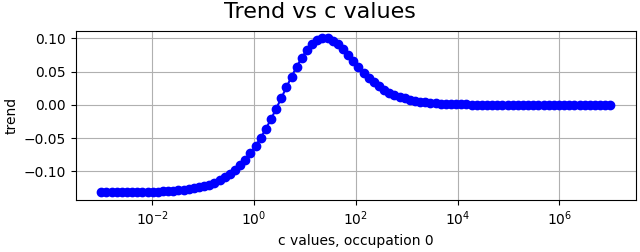
\includegraphics[width=0.7\textwidth]{graphics/data-from-counts-simpson-154}

        \end{center}
    \end{column}%
\end{columns}
\end{frame}

\begin{frame}{Classification algorithms: example from credit default prediction}
  \begin{columns}[T] % align columns
    \begin{column}{.48\textwidth}
      Artificial credit scoring data sample:
      \newline\newline
      \begin{tabular}{rrr}
    \toprule
    default & gender & occupation \\
    \midrule
    0 & 1 & 1 \\
    0 & 0 & 1 \\
    0 & 0 & 1 \\
    1 & 0 & 1 \\
    1 & 0 & 1 \\
    1 & 0 & 0 \\
    0 & 1 & 0 \\
    1 & 1 & 0 \\
    \bottomrule
\end{tabular}\newline\newline
    \end{column}%
    \begin{column}{.48\textwidth}
      Binary target
      \newline\textbf{default}: 0 for no-default, 1 for default
      \newline\newline
      Binary features
      \newline \textbf{gender}: 0 for female, 1 for male \footnote{
        Some current and future credit data will likely have a non-binary gender category.
    } \newline
    \newline \textbf{occupation}: 0, 1 for occupation grouping \newline
    % \textbf{activity}: 0 for low account activity, 1 for high account activity \newline

        % \begin{tabular}{rr}
\toprule
 days &      prob \\
\midrule
    0 &  0.555426 \\
    1 &  0.409581 \\
    2 &  0.274834 \\
    3 &  0.196311 \\
\bottomrule
\end{tabular}
\newline \newline
    \end{column}%
\end{columns}
\end{frame}

\begin{frame}{Classification algorithms: class prediction and scoring functions}

  Given input (``feature'') data $X$ and target (binary) classes $\{0, 1\}$, a \emph{classification} model is a mapping

  \begin{equation*}
    f(X) \in \{0, 1\}
  \end{equation*}

  BUT ... under (almost) all classification algorithms is a function

  \begin{equation*}
    \tilde{f}(X) \in \mathbb{R}^n
  \end{equation*}

  with class membership determined by choosing a threshold $t$ e.g. for binary classification

  \[
 f(X) =
  \begin{cases}
   0 & \text{if } \tilde{f}(X) \leq t \\
   1 & \text{if } \tilde{f}(X) > t
  \end{cases}
\]

Note: if $\tilde{f}(X) \in [0, 1]$, can consider $\tilde{f}$ as a \emph{probability}, but relative values matter (more) in practice, as per \href{https://www.imdb.com/title/tt0088258/}{This is Spinal Tap} scene \href{https://www.youtube.com/watch?v=4xgx4k83zzc}{``These go to 11.''}
\end{frame}

\begin{frame}{Classification trends}
  Let
\begin{itemize}
  \item $(Y,X)$ be a dataset obtained from a $2\times 2\times 2$ contingency table, representing binary random variables $X_1$, $X_2$ and $Y$,
  \item $f_{\beta}$ be a regression model with weights $\beta$, with $\hat{\beta}$ be the fitted weight estimate,
\end{itemize}

% For a regression model $f_{\beta}$ with weights $\beta$, let $\hat{\beta}$ be the weight estimate.

% For binary input events $(X_1 = j, X_2 = k)$, we obtain a score by evaluating $f_{\hat{\beta}}$ at the vector $(j~k)^T$ and denote it by $f_{\hat{\beta}}(X_1 = j, X_2 = k)$.

\begin{definition}
    The \emph{trend indicator} for the subpopulation $X_i = a$ (more generally `event') (for $i\in\{1,2\}$) is
    \begin{equation}
        \label{equ:trendIndicator}
        \T_{X_i=a} = f_{\hat{\beta}}(X_{\bar{i}} = 0, X_i = a) - f_{\hat{\beta}}(X_{\bar{i}} = 1, X_i = a).
    \end{equation}
    Here, $\bar{i}$ denotes the value in $\{1,2\}$ different from $i$.
\end{definition}
\vspace{0.5cm}

Running example: $f_{\hat{\beta}}(X_1=0, X_2 = 0) = 2$, $f_{\hat{\beta}}(X_1=1, X_2=0) = 4$, so $\T_{X_2=0} = 4 - 2 = 2$ \newline
$\rightarrow$ Women in occupation group 0 are less likely to default men.

\end{frame}

\begin{frame}{Ridge regression and regularization}
  Ridge regression is a version of linear regression introducing a penalization term for the parameters to prevent overfitting \cite[\S 3.4.1]{hastie2009elements}.

  Let $X$ be of size $N\times p$ and $Y$ by $N$-dimensional response variable.

  The \emph{regression estimator} is a $p$-dimensional vector $\hat{\beta}$ solving
\begin{equation*}
    \label{equ:optimizationRR}
    \hat{\beta}(c) = \underset{\beta\in\R^p}{\argmin}~ ||Y - X\beta||^2_2 + c||\beta||^2_2.
\end{equation*}
Here, $c\in\R_{>0}$ is the \emph{regularization parameter} controlling the strength of the regularization. In the limit case $c\rightarrow 0$, ridge regression becomes ordinary linear regression.
\end{frame}

\begin{frame}{Logistic regression and regularization}
  Let $X$ be of size $N\times p$ and $Y$ by $N$-dimensional response variable.

  The \emph{logistic regression estimator} is a $p$-dimensional vector $\hat{\beta}$ solving
  \begin{align*}
    \label{equ:optimizationLR}
    \hat{\beta}(c) &= \underset{\beta\in\R^p}{\argmin}~ -\frac{1}{N} \left( Y^T \log\left(\frac{1}{1 + e^{-X\beta}}\right) + (1 - Y)^T \log\left(1 - \frac{1}{1 + e^{-X\beta}}\right) \right) \\
    & \hspace{0.5cm} + c||\beta||^2_2
  \end{align*}
\end{frame}

\begin{frame}{Adversarial regularization regimes in words and a picture}
\begin{definition}
  Given a dataset $(Y,X)$ obtained from a $2\times 2\times 2$ contingency table, the \emph{adversarial regularization regime} $\A_{i,j}$ for the outcome $X_i=j$ (for $i,j\in\{1,2\}$) is the (possibly empty) subset $\A_{i,j}\subset \R_{>0}$ such that for any $c\in\A_{i,j}$, the sign of the trend indicator $\sgn(\T_{X_i=j}(c))$ is reversed compared to the true trend $\sgn(\lim_{c^{\prime}\downarrow 0} \T_{X_i=j}(c^{\prime}))$.
\end{definition}

$\rightarrow$ $(Y,X)$ has an adversarial regularization regime if there exist $i,j \in \{1,2\}$ such that $\mathcal{A}_{i,j}$ is non-empty.

\begin{center}
  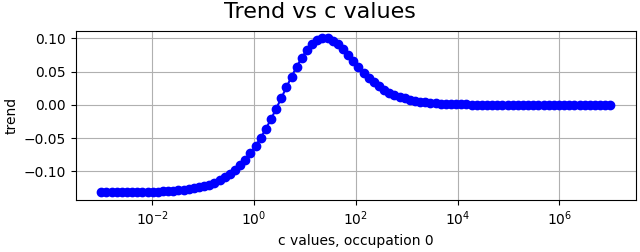
\includegraphics[height=0.3\textheight]{graphics/data-from-counts-simpson-154}
\end{center}

\end{frame}

\begin{frame}{Main results}

  Let $(Y, X)$ be a 2x2x2 random process.\newline

  For ridge regression,
  \begin{itemize}
    \item (Analytical) We find an explicit description of adversarial regularization values.
    \item (Analytical) If $Y \sim \mathrm{Ber}(0.5)$, $X \sim \mathrm{Ber}(0.5)^2$, then probability of a dataset sample of size $N$ has no adversarial regularization values is 0 as $N \rightarrow \infty$.
    \item (Numerical) Among datasets exhibiting Simpson's paradox, the proportion of those having an adversarial regularization regime is $\sim 32\%$ independent of sample size $N$.
  \end{itemize}

For logistic regression,
\begin{itemize}
  \item (Numerical) All datasets exhibiting Simpson's paradox have a non-trivial adversarial regularization regime.
  \item (Numerical) Using k-fold cross validation and weight-balancing mitigates but does not eliminate adversariality
\end{itemize}

\end{frame}

% \begin{frame}{Unpacking main results: Adversarial datasets for ML}
%   Google papers: \cite{szegedy2013intriguing},  \cite{goodfellow2014explaining}

%   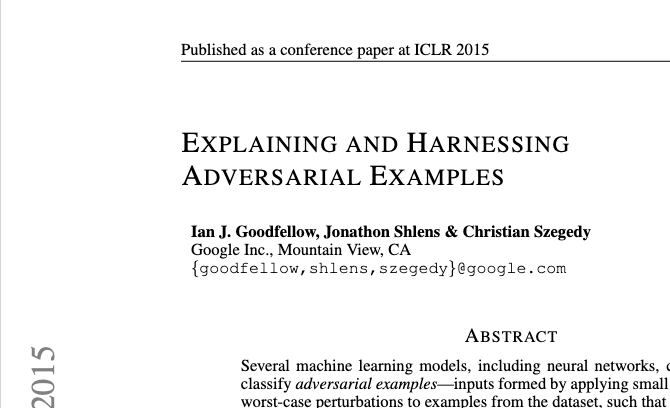
\includegraphics[width=0.7\textwidth]{graphics/explaining-adversarial}
% \end{frame}


% \begin{frame}{Unpacking main results: Adversarial datasets for ML}
%   From \cite{goodfellow2014explaining}\newline
%   \begin{center}
%   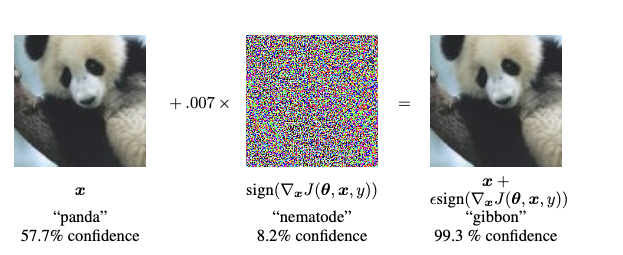
\includegraphics[width=0.7\textwidth]{graphics/gibbon-for-panda}
%   \end{center}

%   \begin{quote}
%     Several machine learning models, including neural networks, consistently mis-
%     classify adversarial examples—inputs formed by applying small but intentionally
%     worst-case perturbations to examples from the dataset, such that the perturbed in-
%     put results in the model outputting an incorrect answer with high confidence.
%     \end{quote}
% \end{frame}

% \begin{frame}{Unpacking the main result: Ridge regression and regularization}
%   Ridge regression is a version of linear regression introducing a penalization term for the parameters to prevent overfitting \cite[\S 3.4.1]{hastie2009elements}.

%   Let $X$ be of size $N\times p$ and $Y$ by $N$-dimensional response variable.

%   The \emph{regression estimator} is a $p$-dimensional vector $\hat{\beta}$ solving
% \begin{equation*}
%     \label{equ:optimizationRR}
%     \hat{\beta}(c) = \underset{\beta\in\R^p}{\argmin}~ ||Y - X\beta||^2_2 + c||\beta||^2_2.
% \end{equation*}
% Here, $c\in\R_{>0}$ is the \emph{regularization parameter} controlling the strength of the regularization. In the limit case $c\rightarrow 0$, ridge regression becomes ordinary linear regression.
% \end{frame}

% \begin{frame}{Unpacking the main result: Logistic regression and regularization}
%   Let $X$ be of size $N\times p$ and $Y$ by $N$-dimensional response variable.

%   The \emph{logistic regression estimator} is a $p$-dimensional vector $\hat{\beta}$ solving
%   \begin{align*}
%     \label{equ:optimizationLR}
%     \hat{\beta}(c) &= \underset{\beta\in\R^p}{\argmin}~ -\frac{1}{N} \left( Y^T \log\left(\frac{1}{1 + e^{-X\beta}}\right) + (1 - Y)^T \log\left(1 - \frac{1}{1 + e^{-X\beta}}\right) \right) \\
%     & \hspace{0.5cm} + c||\beta||^2_2
%   \end{align*}
% \end{frame}

% \begin{frame}{Unpacking the main result: Classification from regression}
%   % \emph{Regression to classification}: interpret its outputs as a score indicative of an input vector $X$ belonging to target output $Y=0$ or $Y=1$. The trend indicator is then the difference between the scores obtained from different binary inputs.\par

% More concretely, let
% \begin{itemize}
%   \item $(Y,X)$ be a dataset obtained from a $2\times 2\times 2$ contingency table, representing binary random variables $X_1$, $X_2$ and $Y$,
%   \item $f_{\beta}$ be a regression model with weights $\beta$, with $\hat{\beta}$ be the fitted weight estimate,
% \end{itemize}let

% % For a regression model $f_{\beta}$ with weights $\beta$, let $\hat{\beta}$ be the weight estimate.

% % For binary input events $(X_1 = j, X_2 = k)$, we obtain a score by evaluating $f_{\hat{\beta}}$ at the vector $(j~k)^T$ and denote it by $f_{\hat{\beta}}(X_1 = j, X_2 = k)$.

% \begin{definition}
%     The \emph{trend indicator} for the input event $X_i = j$ (for $i\in\{1,2\}$) is
%     \begin{equation}
%         \label{equ:trendIndicator}
%         \T_{X_i=j} = f_{\hat{\beta}}(X_i = j, X_{\bar{i}} = 0) - f_{\hat{\beta}}(X_i = j, X_{\bar{i}} = 1).
%     \end{equation}
%     Here, $\bar{i}$ denotes the value in $\{1,2\}$ different from $i$.
% \end{definition}
% \vspace{0.5cm}

% Running example: $f_{\hat{\beta}}(V=0, G = 0) = 2$, $f_{\hat{\beta}}(V=0, G=1) = 4$, so $\T_{V=0} = 4 - 2 = 2$ \newline
% $\rightarrow$ $(V=0, G = 1)$ is more likely to default than $(V=0, G = 0)$
% % $f_{\hat{\beta}}(G = 0, V=0} = 1$
% \end{frame}

\begin{frame}{Really adversarial?}

Simpson datasets occur both
\begin{itemize}
  \item university admissions \cite{Bickel398}, clinical trials \cite{ABRAMSON19921480}, death penalty decisions vs race \cite{radelet1981racial}
  \item in theory: probability of sampling a probability distribution exhibiting Simpson's paradox is $\sim 1.7\%$ \cite{hadjicostas1998asymptotic}
\end{itemize}


\end{frame}


\begin{frame}{Another reason to beware of a \emph{Minority Report}-like future}
  Recall \emph{high risk} AI from
  \begin{columns}[T] % align columns
    \begin{column}{.48\textwidth}
      
\includegraphics[width=0.7\textwidth]{graphics/wikimedia-Minority_Report_Poster}
      \cite{minority-report-poster}
    \end{column}%
    \begin{column}{.48\textwidth}
      Death penalty data from \cite{radelet1981racial}, feature data $X$ corresponding to race of victim and defendant, target $Y$ given death penalty or not: Simpson dataset $\rightarrow$ adversarial for ridge regression.
    \end{column}%
\end{columns}

\end{frame}

\begin{frame}[allowframebreaks]
  \frametitle{References}
  \setbeamertemplate{bibliography item}[text]
  \bibliographystyle{amsalpha}
  \bibliography{../references.bib}
\end{frame}

\end{document}